\chapter{Laboratorio 1: \\Power Estimation: probabilistic techniques}
\section{Probability and Activity Calculation: Simple Logic Gates}
Durante la prima parte dell'esercitazione è stata calcolata la probabilità di avere '1' logico in uscita di alcuni gate elementari, con la relativa Switching Activity.
\begin{figure}[!htb]
	\centering
	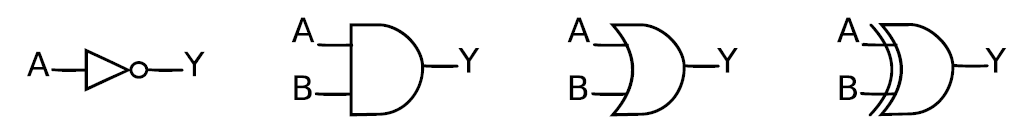
\includegraphics[scale=0.8]{immagini/gate}
	\caption{\textit{Probabilità e Switching Activity stimati manualmente}}
	\label{fig1_1}
\end{figure} \\
La probabilità di '1' logico è stata stimata semplicemente andando a valutare il rapporto fra il numero di possibili combinazioni con '1' logico diviso il numero di combinazioni totali. Invece per il calcolo della Switching Activity è stata utilizzata la formula vista a lezione:
\begin{center}
	$ A=P_{1}P_{0}+P_{1}P_{0}=2P_{1}(1-P_{1}) $
\end{center}
Dove $P_{1}$ e $P_{0}$ sono le probabilità di avere '1' e '0' logici in uscita dalla mia porta. \\
In seguito, tramite il programma \textit{ModelSim} è stato analizzato il numero di toogle delle varie porte utilizzando un testbench sviluppato appositamente dai docenti. Si è andato a variare il numero di colpi di clock, come richiesto dalla traccia ed in seguito si sono comparati i valori ottenuti dalla simulazione con ciò che si era calcolato manualmente.\\
Tramite appositi comandi di Modelsim (\textbf{-power report}), sono stati stilati dei report relativi ad una stima delle commutazioni delle varie porte, della quale se ne riporta un esempio in Figura \ref{fig1_2}. Questi report consentono di stimare l'attività delle porte come verrà descritto in seguito.\\
\begin{figure}[!htb]
	\centering
	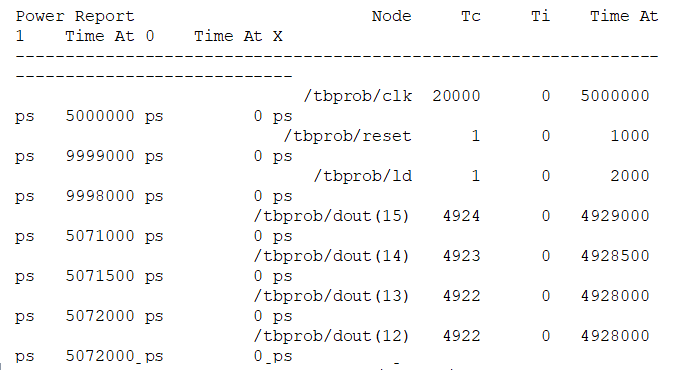
\includegraphics[scale=1]{immagini/fig1_2}
	\caption{\textit{Probabilità e Switching Activity stimati manualmente}}
	\label{fig1_2}
\end{figure} \\
Si riportano nella tabella \ref{tab1}, i risultati ottenuti dalle varie simulazioni.
\begin{table}[!h]\footnotesize
	\centering
	\begin{tabular}{|c|c|c|c|c|}
		\hline
		\textbf{Tc(CK)} & \textbf{Tc(INV)}& \textbf{Tc(AND)}& \textbf{Tc(OR)} &\textbf{Tc(XOR)}\\
		\hline
		20 & 1  & ?& 4&4\\
		\hline
		200 &  43 &40&42& 44\\
		\hline
		2000& 533& 418&352&470\\
		\hline
		20000& 4916& 3606&3784&4876\\
		\hline
	\end{tabular}
	\caption{\textit{Risultati simulazione}}
	\label{tab1}
\end{table}\\
Dai seguenti valori è facile ricavare i valori di Switching Activity simualte, in quanto si possono stimare da:
\begin{center}
	$ A=\frac{Tc(PORT)}{T_{CLK}} $
\end{center}
Come ci si aspettava, essendo la Switching Activity il numero di toogle avvenuti in un periodo, i valori delle simulazioni vengono molto simili ai valori calcolati analiticamente. Aumentando il tempo di simulazione, i valori di Switching Activity diventano sempre più precisi, arrivando ad avere un errore tra 0,01-0,5.

\section{Probability and Activity Calculation: Half and full adder}
Per prima cosa sono state calcolate le probabilità di avere un '1' logico sull'uscita sia dell'half adder e sia del full adder e le probabilità di avere un '1' logico come carry out degli stessi blocchi. Una volta eseguiti questi calcoli sono state calcolate anche le corrispettive switching activity.
\begin{figure}[!htb]
	\centering
	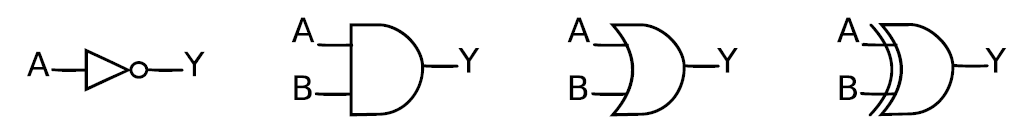
\includegraphics[scale=0.8]{immagini/gate}
	\caption{\textit{Probabilità e Switching Activity stimati manualmente}}
	\label{fig2_1}
\end{figure} \\
La probabilità di '1' logico è stata stimata semplicemente andando a valutare il rapporto fra il numero di possibili combinazioni con '1' logico diviso il numero di combinazioni totali. Invece per il calcolo della Switching Activity è stata utilizzata la formula vista a lezione:
\begin{center}
	$ A=P_{1}P_{0}+P_{1}P_{0}=2P_{1}(1-P_{1}) $
\end{center}
$\alpha$
Dove $P_{1}$ e $P_{0}$ sono le probabilità di avere '1' e '0' logici in uscita dalla mia porta. \\
In seguito, si sono calcolate sempre manualmente le probabilità di uscita con le rispettive switching activity del Ripple carry adder, valutando la probabilità per ogni singolo Half adder come riportato in figura. Per questo calcolo iniziale gli ingressi sono stati considerati scorrelati ed equiprobabili.
\begin{figure}[!htb]
	\centering
	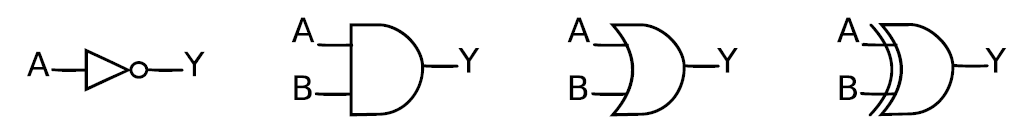
\includegraphics[scale=0.8]{immagini/gate}
	\caption{\textit{Probabilità e Switching Activity stimati manualmente con ingressi equiprobabili}}
	\label{fig2_2}
\end{figure} \\
Nel secondo caso, invece, gli ingressi sono stati considerati sempre scorrelati ma con probabilità diverse, infatti si ha che:
\begin{center}
	$ P(A='1')=0.4 e P(B='1')=0.6 $
\end{center}
I risultati ottenuti risultano uguali ai precedenti, per quanto riguarda la probabilità dell'uscita e del carry out.
In seguito, tramite il programma \textit{ModelSim} è stato simulato il Ripple carry adder (giusto?) utilizzando un testbench sviluppato appositamente dai docenti.Il testbench è stato costruito appositamente per assegnare ritardi diversi al bit di somma, DRCAS, e al bit di carry, DRCAC. Inoltre per garantire una simulazione generale si è utilizzato l'LFSR per generare ingressi randomici.Per una corretta visualizzazione dei risultati si è impostata una risoluzione di 1ps.Dopo aver visualizzato il power report, come fatto già in precedenza, si sono comparati i valori ottenuti dalla simulazione con ciò che si era calcolato manualmente, seguendo lo stesso ragionamento del punto precedente.\\
	\begin{figure}[!htb]
		\centering
		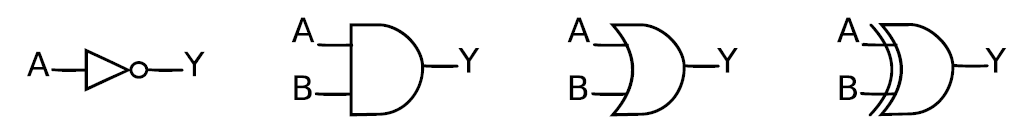
\includegraphics[scale=1]{immagini/gate}
		\caption{\textit{Power report}}
		\label{fig1_3}
	\end{figure} \\
	(cosa noto?) e bisogna mettere le waveforms?\\                                <- ATTENZIONE
Si è poi simulato il caso in cui i due ritardi riguardanti il bit di somma e il bit di carry fossero uguali, e anche per questo è stato visualizzato il power report.   
\begin{figure}[!htb]
		\centering
		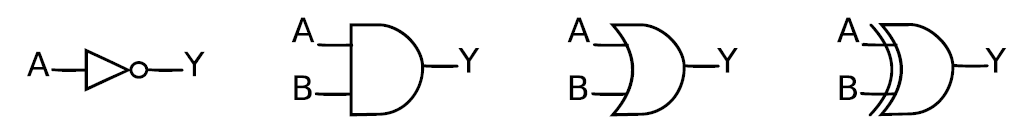
\includegraphics[scale=1]{immagini/gate}
		\caption{\textit{Power report con ritardi uguali}}
		\label{fig1_4}
	\end{figure} \\
	Da un analisi e confronto tra i risultati ottenuti manualmente e quelli ottenuti con le simulazioni, si nota come questi coincidano dato che avendo uguali ritardi, non riesco a simulare la presenza di eventuali glitch.\\
	In seguito si è calcolata la switching activity totale dei due sommatori, utilizzanso la seguente formula:
	\begin{center}
		$ A=\sum_{i=1}^{N-1}{A(S_i)} $  %<- risultato??
	\end{center}
What is the overhead computation of the second adder?  $<$- cioè? \\
Come ultima cosa è stato simulato il secondo testbench che ci è stato fornito, dove si simulava sempre un Ripple carry adder, ma questa volta in maniera puramente combinatoria.Analizzando i risultati, si può concludere come non avendo un segnale di temporizzazione, lavoro alla massima velocità ma ho la presenza di glitch.

\section{RCA synthesis and power analysis}
Nella seguente sezione dell'esercitazione è stata analizzata la potenza del sommatore RCA già analizzato in precedenza, tramite il software \textit{Synopsys}. Dopo aver analizzato ed elaborato i file che descrivono la struttura dell'RCA, il tutto è stato sintetizzato e sono stati raccolti i vari report relativi alla potenza.
Un primo report di potenza, riportato in Figura \ref{report_power1}, descrive i contributi di potenza relativi alle 8 istanze dei Full-Adder che compongono il somamtore RCA. \\
\begin{figure}[!htb]
	\centering
	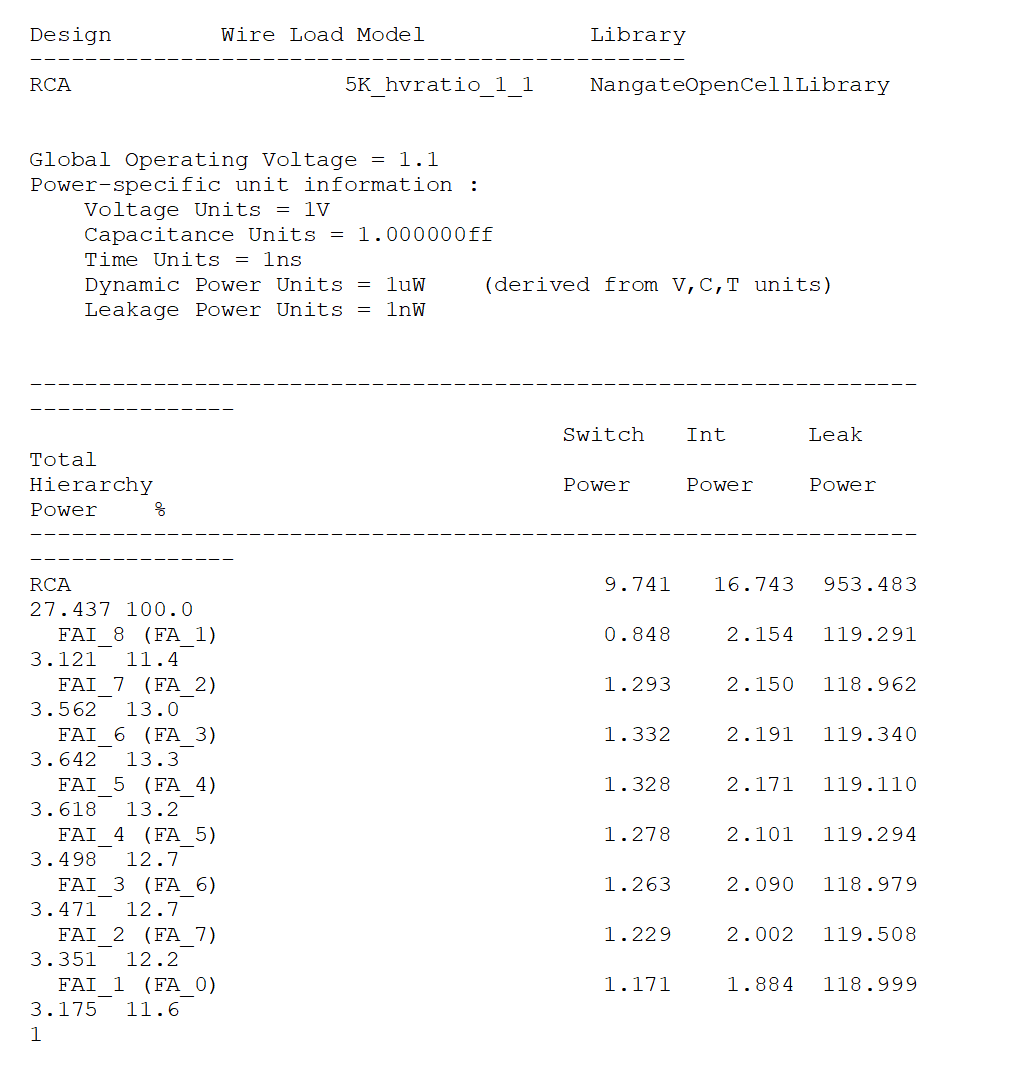
\includegraphics[scale=0.7]{immagini/report_power1}
	\caption{\textit{Power report}}
	\label{report_power1}
\end{figure}
Come ci si aspettava, i contributi dei vari Full Adder sono tutti simili tra di loro, ad eccezione dell'istanza \textit{FAI\_8}: il motivo consiste nel fatto che il Carry Out dell'ultimo Full Adder non è connesso a nessun altra porta, dunque il carico da pilotare è decisamente minore.\\
Diventa ora interessante andare ad analizzare la singola istanza, per andare a valutare l'origine dei singoli contributi di potenza. Tramite il comando \textit{current\_instance FAI\_1} vado ad analizzare l'istanza relativa al primo Full Adder. Viene riportato il report in Figura \ref{reportFA1}.\\
\begin{figure}[!htb]
	\centering
	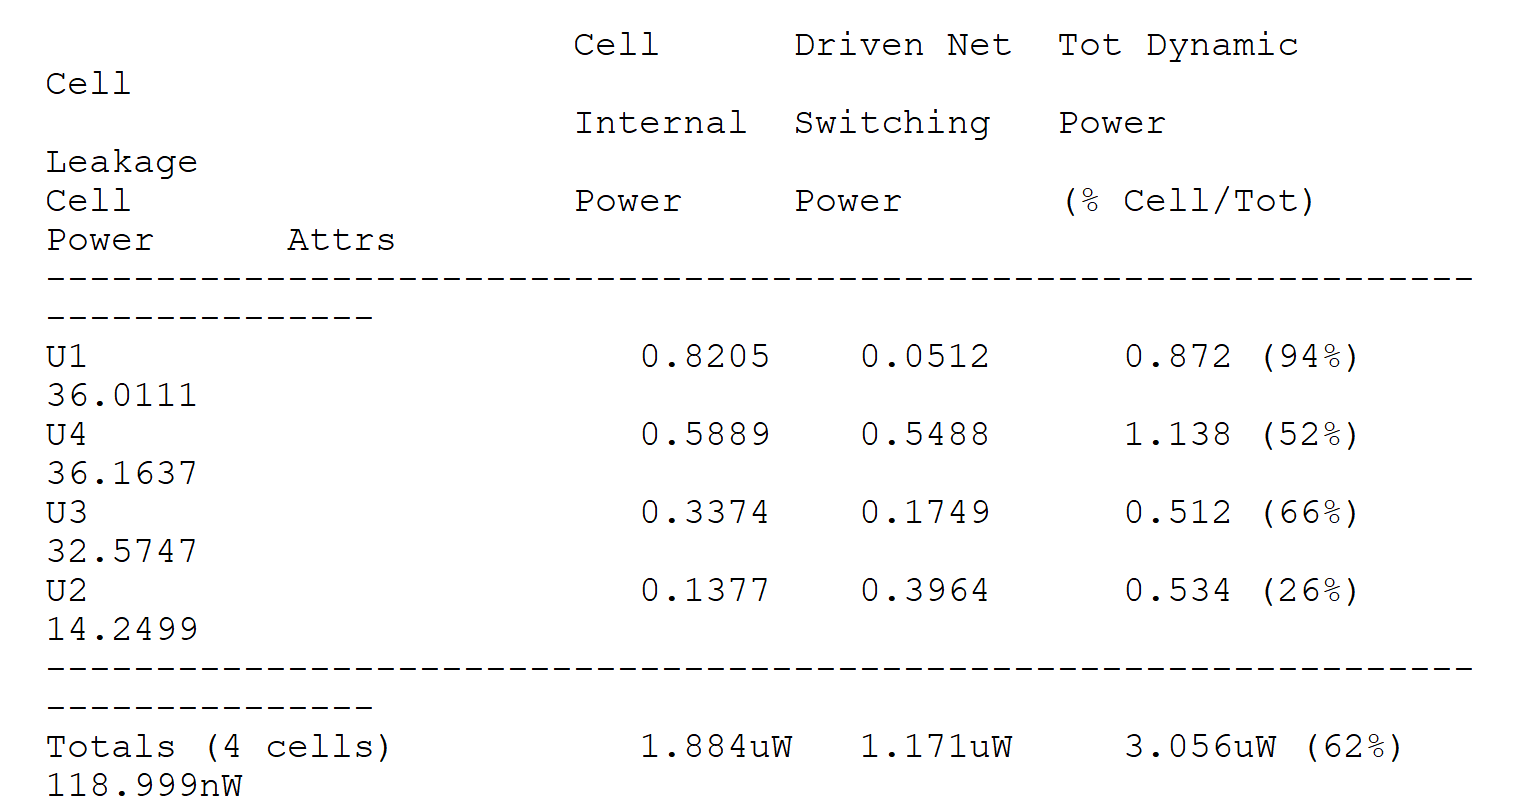
\includegraphics[scale=0.6]{immagini/reportFA1}
	\caption{\textit{Power report}}
	\label{reportFA1}
\end{figure}
Come ci si aspettava i valori di potenza risultano assolutamente identici al report trovato in precendenza e riportato in Figura \ref{report_power1}.
Il passo finale è comprendere come avvenga la stima della potenza dinamica (\textit{switching power}) dei singoli nodi del FA

\section{RCA synthesis and power analysis}